% === Revised Section 5: Solomonoff induction ===
%
% NEW PREAMBLE ADDITIONS NEEDED:
% ---------------------------------------------------------------
% \usepackage{tikz}
% \usepackage{pgfplots}
% \pgfplotsset{compat=1.17}
% \usepackage{listings}
% \lstset{
%   basicstyle=\ttfamily\small,
%   breaklines=true,
%   columns=fullflexible,
%   frame=single,
%   xleftmargin=4pt,
%   xrightmargin=4pt,
% }
%
% \newtcolorbox{activity}[1][]{
%   breakable,
%   enhanced,
%   colback=green!6,
%   colframe=green!45!black,
%   coltitle=white,
%   fonttitle=\bfseries,
%   title={Activity},
%   boxrule=0.6pt,
%   left=6pt,right=6pt,top=4pt,bottom=4pt,
%   #1
% }
% ---------------------------------------------------------------

\section{Solomonoff induction}
\label{sec:solomonoff}

\begin{intuition}
To predict the future, average the predictions of every possible
theory, giving shorter theories exponentially more weight
(\cref{def:M,thm:solomonoff}).

\textbf{The prediction-market analogy.}  Imagine a prediction market
where every trader is a theory of the world.  Simple theories start
with a large float; complex theories start with almost nothing ---
their share price is their \emph{simplicity premium}, set by theory
length: a theory of length $L$ bits gets weight $2^{-L}$.  A theory
you can state in $10$ bits gets a float $2^{10}=1024$ times larger
than one needing $20$ bits.  Each new data point is an earnings call.
Theories that predicted it cheaply get paid; theories that predicted
it badly get margin-called.  Over time the market consolidates around
the simplest theories that still explain the tape.  That
consolidation \emph{is} the Solomonoff prediction $M$.  This is
Occam's razor, precisely quantified: ``precisely'' meaning that the
trade-off between fit and simplicity is not an aesthetic preference
but a \emph{probability} with a formula.

\textbf{Occam as an airline fee.}  Think of the prior as a
business-class airline that charges \$2 of prior mass for every extra
byte of theory you pack.  A $10$-byte theory boards for
\$$2^{10}\!\approx\!\$1024$ (measured in inverse prior), a $20$-byte
theory for \$$2^{20}\!\approx\!\$1{,}048{,}576$.  Fit-to-data is the
voucher that reimburses you; over- fitters, who smuggled in extra
bytes just to match noise, never recover the fee.

\textbf{A tiny worked example (same universe as \cref{ex:toy-solomonoff}).}
Two theorists compete: $\pi_0$ says ``always $0$'' ($2$ bits long),
$\pi_1$ says ``alternate $0101\dots$'' ($3$ bits long).  Before data,
$\pi_0$ holds $2/3$ of the prior float, $\pi_1$ holds $1/3$.  You
observe the bit $0$: both theorists predicted it, so the ratio is
unchanged.  You observe another $0$ (sequence so far $00$): still
consistent with both, so again unchanged.\footnote{$\pi_1$ predicts
$01$ deterministically, so in fact $00$ already falsifies $\pi_1$ ---
we gloss this for rhetorical rhythm and restore it in the formal
example.}  The moment you see a $1$, $\pi_0$ is margin-called to
zero and $\pi_1$ inherits the entire float.  One bit of the right
kind can collapse a prior --- that is what makes Solomonoff
\emph{fast}.

\textbf{Convergence, in plain English.}  If the true process is
computable, Solomonoff's predictor converges to it: the total
``surprise'' it will ever suffer, summed over all future time steps,
is bounded by the length (in bits) of the shortest program that
describes the true process.  A decision-maker's translation: you pay,
\emph{once}, a number of bits equal to the complexity of the truth;
after that, the predictor is free.

\textbf{Bayesian model averaging, without the jargon.}  ``Bayesian
model averaging'' is the generic name for: keep a zoo of hypotheses,
weight each by how well it predicted the past, average their
predictions for the future.  Solomonoff is the limiting case where
the zoo is ``every computable hypothesis'' and the prior weight is
$2^{-\text{length}}$.

Why a decision-maker should care: Solomonoff induction is the gold
standard of ``learning from data.''  Every ML method is, badly and
efficiently, trying to imitate it.  ``Ensemble methods'' and
``regularise for simplicity'' are engineering approximations of this
ideal.  It also explains why overfitting is bad in a principled way:
an overfit model is a long, ad-hoc theory, and Solomonoff would have
weighted it near-zero from the start.  The question ``which model is
best?'' has a right answer: whichever predicts held-out data with the
fewest bits of surprise.
\end{intuition}

\subsection*{From intuition to definition}

Kolmogorov complexity selects a \emph{single} shortest program.
Solomonoff's prior \citep{solomonoff1964formal} performs a
\emph{Bayesian average} over \emph{all} programs, weighted by their
lengths.  Concretely: fix a \emph{prefix-free} universal Turing
machine $U$.  ``Prefix-free'' just means that no valid program is a
prefix of another valid program --- the same property that makes
Morse code or Huffman codes unambiguous.  For such a machine, the
set of halting inputs forms a prefix code, so the total prior mass
is at most one:
\[
  \sum_{\pi : U(\pi)\downarrow} 2^{-|\pi|} \;\le\; 1
  \qquad(\text{Kraft's inequality}).
\]
A one-line sanity check: if each program of length $L$ were given
weight $2^{-L}$ and there were $2^L$ of them at each length,
the total would diverge.  Kraft's inequality says the prefix-free
property prunes enough programs to keep the sum finite, and indeed
$\le 1$; it therefore defines a genuine probability distribution.

\begin{definition}[Universal prior $M$]
\label{def:M}
For a finite binary string $x \in \{0,1\}^*$, the \textbf{universal
(Solomonoff) prior} is
\begin{equation}
  M(x) \;=\; \sum_{\pi \,:\, U(\pi)\, =\, x *} 2^{-|\pi|},
  \label{eq:M}
\end{equation}
where the sum runs over all programs $\pi$ such that $U(\pi)$ halts
and outputs a string whose prefix is $x$ (denoted $x*$).
Equivalently, $M(x)$ is the probability that $U$, fed with a
uniformly random infinite bitstream, prints $x$ as its first $|x|$
output bits.
\end{definition}

\noindent The Solomonoff predictive posterior is obtained, as with any
probability distribution, by conditioning:
\begin{equation}
  M(x_{t+1} \mid x_{1:t}) \;=\; \frac{M(x_{1:t}\,x_{t+1})}{M(x_{1:t})},
  \label{eq:M-posterior}
\end{equation}
defined whenever $M(x_{1:t}) > 0$.  Every ML system that ``updates on
data'' is, secretly, approximating this ratio.

\begin{activity}[Classroom prediction market --- 5 rounds, 10 min]
\label{act:prediction-market}
\textbf{Props.}  One bag of 64 poker chips per group of 5 students; a
whiteboard; five index cards each labelled with a candidate
``theory'' for the sequence about to be generated.

\textbf{Setup.}  Write on the whiteboard five candidate rules for a
binary sequence: \\
$H_1$: all zeros (length $2$, weight $2^{-2}=16$ chips); \\
$H_2$: all ones (length $2$, weight $16$ chips); \\
$H_3$: alternating $0101\ldots$ (length $3$, weight $8$ chips); \\
$H_4$: alternating $1010\ldots$ (length $3$, weight $8$ chips); \\
$H_5$: i.i.d.\ fair coin (length $4$, weight $4$ chips). \\
(Chip counts $16+16+8+8+4=52$; keep the remaining $12$ chips in the
``other theories'' reserve to make the prefix-free bookkeeping
honest.)

\textbf{Play.}  Instructor secretly picks one of the five rules and
generates one bit at a time.  After each bit, any $H_i$ that
deterministically contradicted the observed bit surrenders all its
chips to the reserve; the survivors keep theirs.  For $H_5$, halve
its chip count every round (the i.i.d.\ likelihood of any specific
bit is $1/2$).  After 5 rounds, renormalise: the remaining chips are
the posterior weights.

\textbf{Debrief.}  Students see (a) the shortest surviving theory
usually dominates; (b) a single contradicting bit \emph{instantly}
zeroes a deterministic hypothesis, matching
\eqref{eq:M-posterior}; (c) if the true rule was the i.i.d.\ coin,
its survival is slow but steady --- simplicity dominates early,
fidelity to the data wins late.
\end{activity}

\begin{theorem}[Solomonoff's convergence theorem]
\label{thm:solomonoff}
Let $\mu$ be any computable probability measure on $\{0,1\}^\infty$.
Then there is a constant
\begin{equation}
  c_\mu \;=\; 2^{-K(\mu) + O(1)}
  \label{eq:cmu}
\end{equation}
such that, for all finite prefixes $x$,
\begin{equation}
  M(x) \;\ge\; c_\mu \cdot \mu(x).
  \label{eq:dominance}
\end{equation}
Consequently, if $X_{1:\infty} \sim \mu$, the cumulative expected
KL divergence between the Solomonoff predictor and $\mu$ is bounded
uniformly:
\begin{equation}
  \sum_{t=1}^{\infty}
    \mathbb{E}_{\mu}\!\left[
      D_{\mathrm{KL}}\!\bigl(\mu(\cdot \mid X_{<t}) \,\|\, M(\cdot \mid X_{<t})\bigr)
    \right]
  \;\le\; K(\mu)\ln 2 + O(1).
  \label{eq:sol-bound}
\end{equation}
In particular,
$D_{\mathrm{KL}}(\mu(\cdot \mid X_{<t}) \| M(\cdot \mid X_{<t})) \to 0$
in $\mu$-expectation as $t \to \infty$.
\end{theorem}

\paragraph{Reading \eqref{eq:cmu}--\eqref{eq:sol-bound} in plain
English.}  Inequality \eqref{eq:dominance} says the universal prior
never underestimates the truth by more than a \emph{constant} factor
$c_\mu$, and that constant is exactly the prior mass the truth
deserves: $2^{-K(\mu)}$.  Inequality \eqref{eq:sol-bound} says the
\emph{total} surprise $M$ will accumulate, across all future time
steps, is at most $K(\mu)$ bits (with $\ln 2$ converting bits to
nats).  A fair coin has $K(\mu)$ around 20 bits on a reasonable
reference machine.  A Markov chain whose source code is 100 bytes
has $K(\mu) \le 800$ bits.  Either way the regret is bounded by a
\emph{constant that does not grow with the data} --- a property no
finite-model learner can match without cheating.

\begin{proof}[Proof sketch]
Because $\mu$ is computable, it has a description as a program
$\pi_\mu$ of length $|\pi_\mu| = K(\mu) + O(1)$.  Any program that,
given $\pi_\mu$ as a subroutine, simulates a $\mu$-sample and outputs
a string beginning with $x$ contributes at least
$2^{-K(\mu)-O(1)}\,\mu(x)$ to $M(x)$; summing gives
\eqref{eq:dominance}.  For the KL bound, the key identity is the
telescoping
\[
  \log \frac{\mu(X_{1:T})}{M(X_{1:T})}
  \;=\; \sum_{t=1}^{T}
    \log \frac{\mu(X_t \mid X_{<t})}{M(X_t \mid X_{<t})},
\]
whose $\mu$-expectation is
$\sum_{t=1}^T \mathbb{E}_\mu [D_{\mathrm{KL}}(\mu_t \| M_t)]$.  The
left-hand side is at most $\log(1/c_\mu) = K(\mu) + O(1)$ bits by
\eqref{eq:dominance} and a Jensen step, which in nats is
$K(\mu)\ln 2 + O(1)$.  The correct program $\pi_\mu$ has prior mass
exactly $2^{-K(\mu)}$; the finite KL budget is the
information-theoretic price of identifying it.  For the full proof
see \citet[Ch.~5]{livitanyi2019}.
\end{proof}

\subsection*{A two-program universe, updated step by step}

We now carry out the minimal example in full, because no amount of
prose substitutes for watching a posterior move.

\begin{example}[Toy Solomonoff update on a two-program universe]
\label{ex:toy-solomonoff}
Restrict the universe of programs to two deterministic generators:
$\pi_0 : \text{always output }0$ (bit-length $|\pi_0| = 2$) and
$\pi_1 : \text{output the cycle } 01010101\ldots$ (bit-length
$|\pi_1| = 3$).  Under the Solomonoff-style weighting
$w(\pi) = 2^{-|\pi|}$, the prior over the two hypotheses is
\[
  P(\pi_0) \;=\; \frac{2^{-2}}{2^{-2} + 2^{-3}} \;=\; \frac{2}{3},
  \qquad
  P(\pi_1) \;=\; \frac{2^{-3}}{2^{-2} + 2^{-3}} \;=\; \frac{1}{3}.
\]

\noindent\emph{Step-by-step update on the prefix $0101$.}

\begin{center}
\begin{tabular}{c|cc|c}
after seeing & $P(\pi_0)$ & $P(\pi_1)$ & predicted next bit \\\hline
(nothing) & $2/3$ & $1/3$ & $P(0)=2/3+1/3\cdot 1=1$ \\
$0$       & $2/3$ & $1/3$ & $P(0)=2/3+0=2/3$; $P(1)=1/3$ \\
$01$      & $0$   & $1$   & $P(0)=1$ (the cycle says $0$) \\
$010$     & $0$   & $1$   & $P(1)=1$ \\
$0101$    & $0$   & $1$   & $P(0)=1$ \\
\end{tabular}
\end{center}

\noindent The decisive moment is bit 2: $\pi_0$ predicted $0$ with
probability $1$ and saw $1$, so its likelihood is zero and Bayes
zeros its posterior.  From that step onward $\pi_1$ owns the entire
posterior, and the Solomonoff predictor behaves as the deterministic
cycle predictor.

Two features worth internalising.  (i) The shorter program $\pi_0$
was \emph{not} favoured after data --- simplicity is a prior
preference overridden by evidence.  (ii) A single contradicting bit
collapses an exponentially-weighted prior to a point mass; this is
the mechanism by which Solomonoff induction converges so fast on
deterministic sources.

\paragraph{Visualisation.}
\Cref{fig:posterior-evolution} renders the two rows of the table as
bars.  The second bit of data is where the entire picture changes.

\begin{figure}[h]
\centering
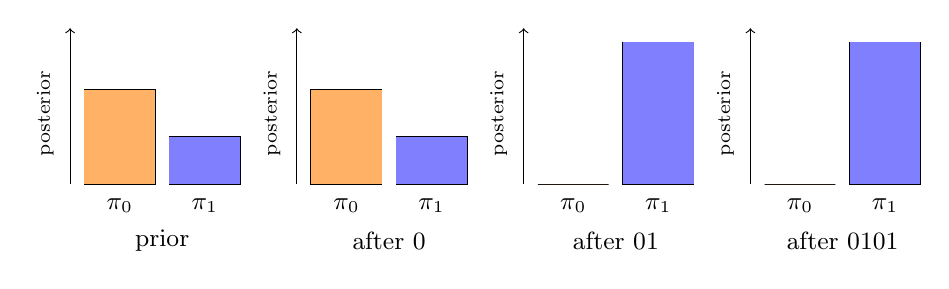
\begin{tikzpicture}[scale=0.9]
  \foreach \t/\p/\q/\lbl [count=\i from 0] in
    {prior/0.667/0.333/{prior},
     0/0.667/0.333/{after $0$},
     01/0.0/1.0/{after $01$},
     0101/0.0/1.0/{after $0101$}} {
    \begin{scope}[xshift=\i*3.2cm]
      \draw (0,0) rectangle (1,2*\p);
      \fill[orange!60] (0,0) rectangle (1,2*\p);
      \draw (1.2,0) rectangle (2.2,2*\q);
      \fill[blue!50] (1.2,0) rectangle (2.2,2*\q);
      \node at (0.5,-0.3) {\small $\pi_0$};
      \node at (1.7,-0.3) {\small $\pi_1$};
      \node at (1.1,-0.8) {\small \lbl};
      \draw[->] (-0.2,0) -- (-0.2,2.2);
      \node[rotate=90] at (-0.55,1.0) {\scriptsize posterior};
    \end{scope}
  }
\end{tikzpicture}
\caption{Posterior mass on the two programs $\pi_0$ (always-zero,
length 2) and $\pi_1$ (alternating, length 3) as the observations
$0,\,01,\,0101$ arrive.  One bit --- the second --- is enough to
collapse the prior to a point mass on $\pi_1$.}
\label{fig:posterior-evolution}
\end{figure}
\end{example}

\begin{activity}[Python: a 6-line Solomonoff predictor]
\label{act:python-solomonoff}
\textbf{Goal.}  Reproduce \cref{ex:toy-solomonoff} and experiment with
other sequences.  Helps build the reflex that ``posterior update ==
multiply by likelihood and renormalise,'' regardless of how
philosophical the prior is.

\begin{lstlisting}[language=Python]
# Two-program Solomonoff toy.
programs = {
    "pi0": {"length": 2, "next": lambda s: "0"},                 # always 0
    "pi1": {"length": 3, "next": lambda s: "01"[len(s) % 2]},    # cycle 01
}
prior = {k: 2 ** (-v["length"]) for k, v in programs.items()}
Z = sum(prior.values()); post = {k: v / Z for k, v in prior.items()}

def update(post, observed_bit, history):
    new = {}
    for k, p in post.items():
        predicted = programs[k]["next"](history)
        new[k] = p if predicted == observed_bit else 0.0
    Z = sum(new.values()) or 1.0
    return {k: v / Z for k, v in new.items()}

history = ""
for bit in "0101":
    post = update(post, bit, history); history += bit
    print(history, post)
\end{lstlisting}

\textbf{Extensions.}  (i) Add a third program $\pi_2$ that outputs
$001001\ldots$ and feed it the sequence $001001$.  (ii) Replace the
deterministic programs with stochastic ones (e.g.\ a $0.6$-biased
coin) and watch the posterior drift rather than collapse.
(iii) Swap the data to $0100$ and observe that \emph{both} programs
die, at which point Solomonoff would fall back on the infinite zoo
we truncated.
\end{activity}

\begin{activity}[Worksheet: which program survives?]
\label{act:fibonacci-worksheet}
\textbf{Given.}  Three candidate programs for a numeric sequence:
\[
  \pi_A : \text{constant }1,\quad
  \pi_B : \text{repeat }1,1,2,\quad
  \pi_C : \text{Fibonacci, } a_{n+2}=a_n+a_{n+1}.
\]
Assign rough bit-lengths $|\pi_A|=6$, $|\pi_B|=10$, $|\pi_C|=15$ (from
their Python source, say).  Compute the prior weights proportional to
$2^{-|\pi_i|}$.  Now observe the sequence
\[
  1,\ 1,\ 2,\ 3,\ 5,\ 8.
\]
\textbf{Tasks.}  (a) After each term, which programs are still
consistent?  (b) Write down the posterior weights at each step.
(c) At what point does $\pi_C$ overtake $\pi_B$ in the posterior?
(d) If the next term is $13$, does your answer change?  What if it
were $13.001$?  (e) The Solomonoff prior contains \emph{every}
computable program.  Which program not on the list would you expect
to be the main ``runner-up'' after seeing $1,1,2,3,5,8$?
\end{activity}

\paragraph{Decision-maker takeaway.}  Solomonoff induction is
uncomputable --- you cannot run $M$ on a real computer --- but it is
the \emph{formal target} that the whole field of machine learning is
approximating.  Every time an ML engineer adds a regulariser, drops
a complicated feature, or averages an ensemble, they are paying
Occam's airline fee from \cref{thm:solomonoff}.  The theorem
guarantees that if they paid it honestly, and if the truth were
computable, their cumulative regret would be finite --- bounded by
the bit-length of the truth.  No method with a finite hypothesis
class can make that promise.  What you \emph{buy} with Solomonoff is
not an algorithm but a benchmark.

% =========================================================================
